\documentclass{article}
\usepackage[UTF8,space,hyperref]{ctex}
\usepackage{amsmath, amsthm, amssymb, bm, color, framed, graphicx, hyperref, mathrsfs, physics, geometry}
\geometry{left=2.0cm,right=2.0cm,top=2.5cm,bottom=2.5cm}

\title{C语言函数传参与返回复杂结构体的机制}
\author{石曜铭}
\date{\today}
\hypersetup{hidelinks}
\geometry{a4paper,scale=0.65}



\begin{document}

\maketitle

\section{实验概述}

本次实验中,我使用 C 语言定义了结构体 Data,并实现传递和返回 Data 类型参数的函数,然后使用编译器编译成汇编代码,通过分析汇编代码中传参和返回值部分的地址偏移量,确定传递复杂类型参数的方式。

此报告中所有汇编语言代码均使用 x86-64 的 AT\&T 语法。

\section{示例代码}
接下来给出实验用到的 C 语言代码。
\begin{figure}[htbp]
    \centering
    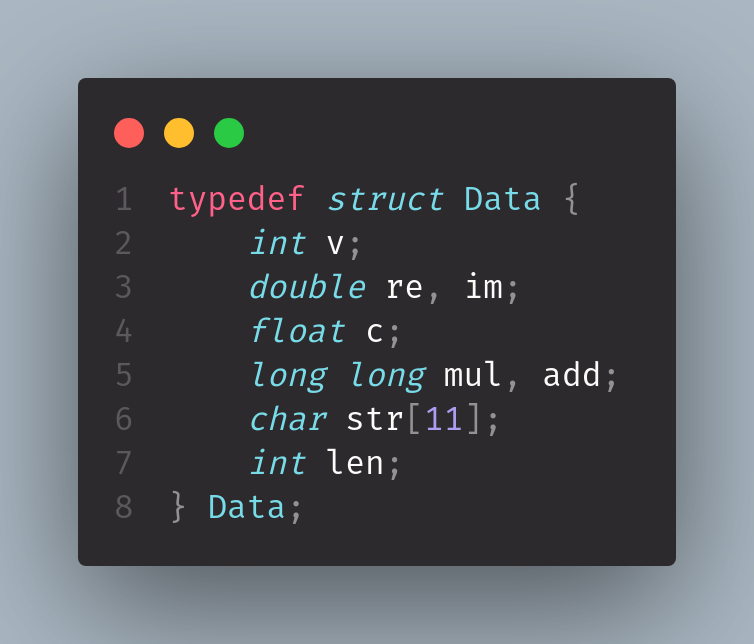
\includegraphics[width=0.5\textwidth]{pics/struct.png}
    \caption{结构体定义}
\end{figure}

结构体 Data 包括 $\texttt{int}$ 类型的 $v$,$\texttt{double}$ 类型的 $re, im$,等其他类型,是一个复杂的数据类型。
\newpage
\begin{figure}[htbp]
    \centering
    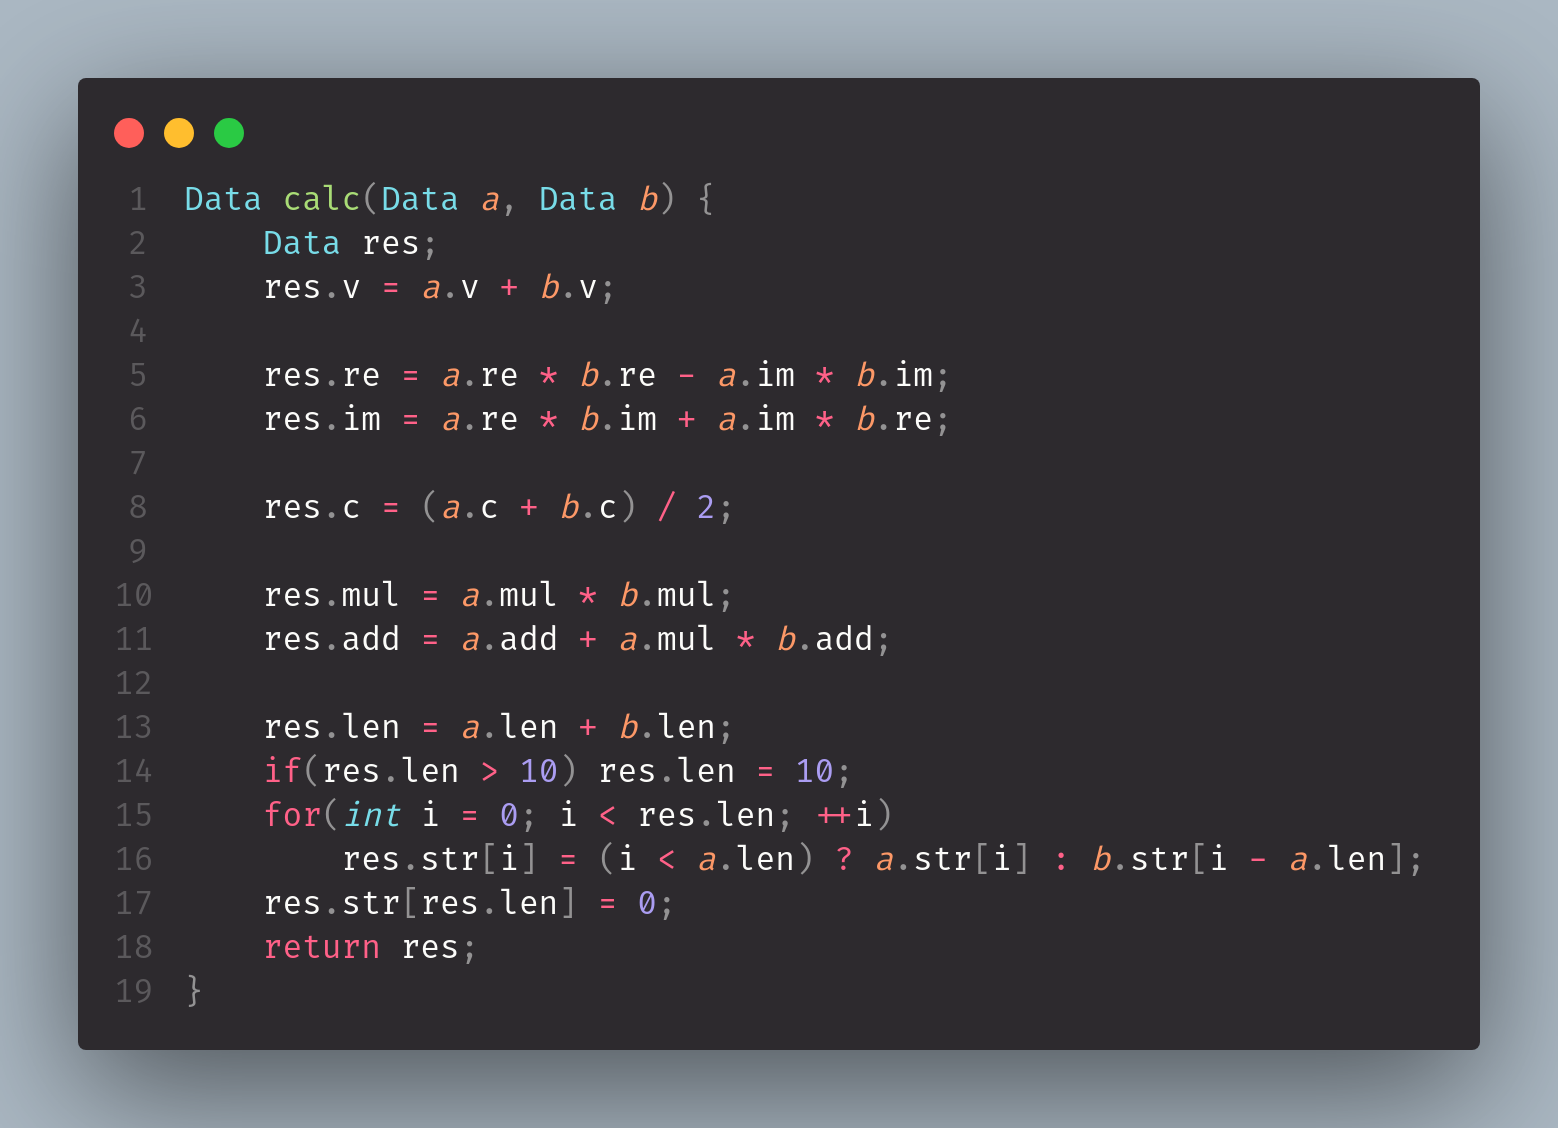
\includegraphics[width=0.8\textwidth]{pics/calc.png}
    \caption{calc 函数定义}
\end{figure}
函数 calc 计算了 $v$ 的加法,复数 $(re,im)$ 的乘法,浮点数 $c$ 的平均数,先乘后加标签的合并,与字符串的拼接。函数需要用到输入的两个 Data 类型的所有成员,计算互不相同,可以在汇编代码中容易区分出是哪一个成员。

\begin{figure}[htbp]
    \centering
    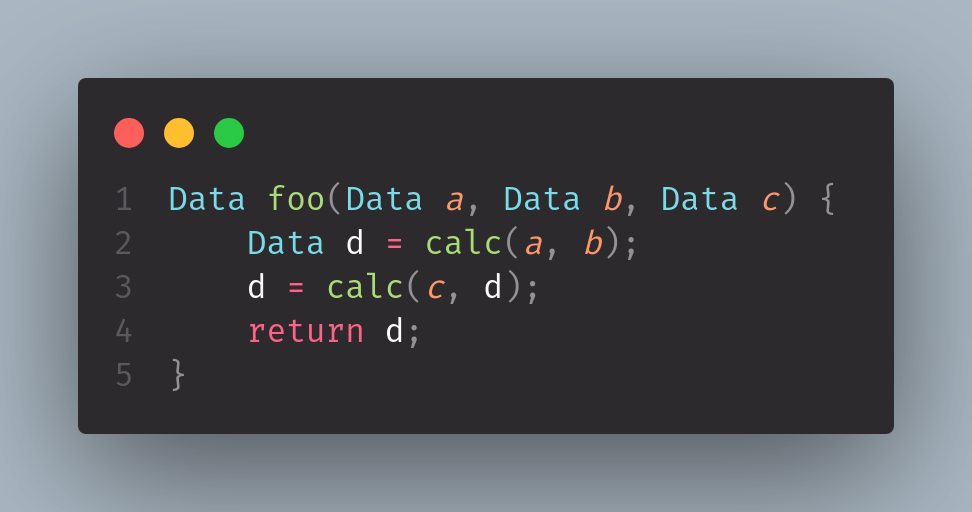
\includegraphics[width=0.6\textwidth]{pics/foo.png}
    \caption{调用 calc 函数示例}
\end{figure}
Data foo(Data a, Data b, Data c):调用calc两次,返回最终结果。


\newpage
\section{参数传递机制分析}
在x86-64架构下,遵循System V ABI调用约定:
\begin{itemize}
\item \textbf{参数传递}
\begin{itemize}
   \item 若结构体大小超过寄存器容量(如16字节),参数通过栈传递。  
   \item 示例中 calc(Data a, Data b) 的两个参数均为大结构体,因此调用者将 $a$ 和 $b$ 的内容依次压入栈中。
   \item 汇编代码中,通过 rbp+偏移量 访问参数成员,例如 movl 16(\%rbp), \%edx,访问 $a$ 的首地址。
\end{itemize}
\item \textbf{返回值传递}
\begin{itemize}
   \item 大结构体无法通过寄存器返回,\textbf{调用者需预先分配内存},并将该内存地址作为隐藏的第一个参数(通过 \%rdi 寄存器)传递给函数。
   \item 函数内部将结果写入该地址,最后返回该地址。  
   \item 示例中 calc 函数的汇编代码:movq \%rdi, -24(\%rbp) 保存返回地址到栈;movq -24(\%rbp), \%rax 加载返回地址;movl \%edx, (\%rax) 写入结果到返回结构体的v成员。
\end{itemize}  
\end{itemize}

\section{汇编代码关键片段解析}
\subsection{calc 函数参数访问}
从代码中可以看到,两个结构体参数在栈上连续存放,通过固定偏移量访问成员。$a$ 的起始位置是 16(\%rbp),$b$ 的起始位置是 80(\%rbp)。

对应代码:

movl 16(\%rbp), \%edx

movl 80(\%rbp), \%eax

\subsection{返回值写入(以成员 re 的计算为例)}
首先获取调用者传入的返回地址:movq -24(\%rbp), \%rax

然后将计算结果写入返回结构体的re成员(偏移8字节):movsd \%xmm0, 8(\%rax)

从中也可以发现 $re$ 成员在结构体对象首地址往后偏移 $8$ 字节的位置。

\subsection{foo 函数调用 calc 时传参的过程}
首先,在栈上分配存放参数的空间:subq \$64, \%rsp 

然后,将栈顶地址作为参数起始地址:movq \%rsp, \%rax 

然后,拷贝结构体成员到栈:movq \%rcx, (\%rax) 

传递返回地址:movq \%rdx, \%rdi 

调用 calc 函数:call calc

综上,调用者需手动拷贝结构体内容到栈,并传递返回地址。



\end{document}